\documentclass[crop=false,10pt,ngerman]{standalone}
\usepackage{standard}
\begin{document}
  \section{Implementierung} % (fold)
  \label{sec:implementierung}

    \subsection{Repräsentation des Berechnungsgebietes} % (fold)
    \label{sub:repräsentation_des_berechnungsgebietes}
      Es handle sich bei $[\domain]\define\roundBrackets{\domain,\dirichletBoundary,\neumannBoundary,ν}$ wieder um ein Berechnungsgebiet.
      Die Implementierung einer Finite-Elemente-Methode verlangt die Diskretisierung von $[\domain]$, wie es in Abschnitt \ref{ssub:discretization-domain} beschrieben wurde.
      Es sei $(V,E,\mathscr{T})$ eine Triangulierung von $[\domain]$.
      Die Implementierung der Basisstruktur für die Triangulierung des Berechnungsgebietes sei durch den folgenden Quelltext gegeben.

      \inputCodeBlock[title=domain\_base]{code/domain_base.cc}
      Die Basisstruktur wird als \code{Domain\_base} im Namespace \code{Fem} konstruiert.
      In ihr werden die Strukturen \code{Edge} und \code{Primitive} für die Beschreibung der Kanten und Dreiecke deklariert.
      Die verschiedenen Konstruktoren und Zuweisungsoperatoren der Sprache C++ werden explizit durch den Compiler erzeugt.
      Der Destruktor wurde mit \code{virtual} gekennzeichnet, wie es für polymorphe Basisklassen angebracht ist \cite[S.~40~ff]{Meyers2008}.

      \inputCodeBlock[title=edge]{code/edge.cc}
      Die Datenstruktur \code{Edge} der Basisklasse \code{Domain\_base} wird durch ein Array von zwei Integern dargestellt.
      Diese verweisen später auf die Eckpunkte der Kante.
      Der Konstruktor stellt sicher, dass die Indizes sortiert übergeben werden.
      Innerhalb der Datenstruktur werden zwei weitere Datenstrukturen \code{Hash} und \code{Info} deklariert, die für die fehlerfreie Konstruktion eines Berechnungsgebietes verwendet werden.
      Die Datenstruktur \code{Primitive} eines Dreiecks ist analog aufgebaut.
      Um die drei Indizes für die Referenzierung auf die Eckpunkte zu sortieren wird hier ein einfaches Insertion sort verwendet.
      \inputCodeBlock[title=primitive]{code/primitive.cc}

      Die eigentliche Datenstruktur \code{Domain} eines Berechnungsgebietes erbt von der Basisklasse \code{Domain\_base}.
      Zudem wird der Datentyp der Eckpunkte durch ein Template variabel gehalten.
      Das Interface der Klasse ergibt sich aus Funktionen, um Daten zu lesen und fehlerfrei hinzuzufügen.
      Um dies auch in der Implementierung zu gewährleisten, werden für das Aufbewahren der Dreiecke und Kanten Hash Maps verwendet.
      Diese speichern, wie oft eines der genannten Objekte zum Berechnungsgebiet hinzugefügt wurde.
      Auf der Basis dieser Zahl ist die Klasse dann in der Lage zwischen Randkanten und inneren Kanten zu unterscheiden und fehlerhafte Berechnungsgebiete zu verhindern.
      \inputCodeBlock[title=domain]{code/domain.cc}
      \inputCodeBlock[title=domain implementation]{code/domain_implementation.cc}

      Für die späteren Messungen ist es von großem Nutzen, die Triangulierung eines Gebietes zu verfeinern.
      Hierfür enthält die Klasse \code{Domain} eine Funktion \code{subdivide}.
      Sie ermittelt für jede vorhandene Kante einen neuen Eckpunkt und fügt dann auf der Basis der alten Dreiecke neue feinere Dreiecke hinzu.
      Die unterteilten Kanten behalten dabei ihre Randeigenschaften.
      \inputCodeBlock[title=subdivide]{code/domain_implementation_subdivide.cc}

      Um ein Berechnungsgebiet außerhalb des Quelltextes leicht zu beschreiben, wurde ein Dateiformat definiert.
      Im folgenden ist ein Beispiel für blabla gezeigt.
      Hierbei steht \code{v} für die Definition eines Eckpunktes, \code{p} für die Definition eines Dreiecks, \code{q} für die Definition eines Vierecks, \code{d} für eine Dirichlet-Kante und \code{n} für eine Neumann-Kante.
      \begin{center}
        \noindent
        \begin{minipage}[b]{0.32\textwidth}
          \begin{tcolorbox}[titlerule=0.1pt,boxrule=0.5pt,arc=5pt,title={Zeile 1-13}]
            \lstinputlisting[style=standard,firstline=1,lastline=13]{code/model-test.txt}
          \end{tcolorbox}
        \end{minipage}
        \hfill
        \begin{minipage}[b]{0.32\textwidth}
          \begin{tcolorbox}[titlerule=0.1pt,boxrule=0.5pt,arc=5pt,title={Zeile 14-26}]
            \lstinputlisting[style=standard,firstline=14,lastline=26]{code/model-test.txt}
          \end{tcolorbox}
        \end{minipage}
        \hfill
        \begin{minipage}[b]{0.32\textwidth}
          \begin{tcolorbox}[titlerule=0.1pt,boxrule=0.5pt,arc=5pt,title={Zeile 27-39}]
            \lstinputlisting[style=standard,firstline=27,lastline=39]{code/model-test.txt}
          \end{tcolorbox}
        \end{minipage}
      \end{center}

      \begin{figure}[h]
        \begin{subfigure}[b]{0.24\textwidth}
          \center
          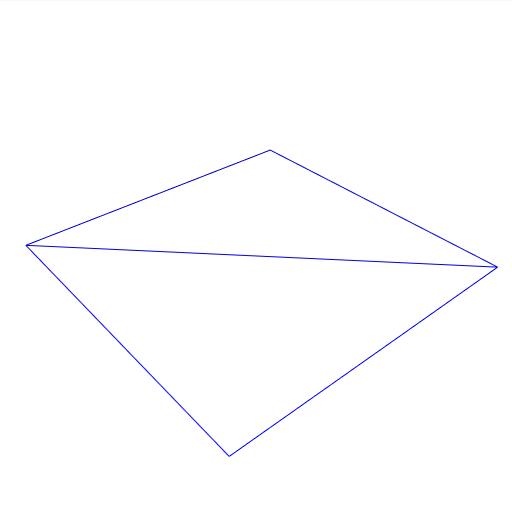
\includegraphics[trim={0 0 0 2cm},clip,width=0.95\textwidth]{images/model-quad-0.png}
          \caption{Quad}
        \end{subfigure}
        \begin{subfigure}[b]{0.24\textwidth}
          \center
          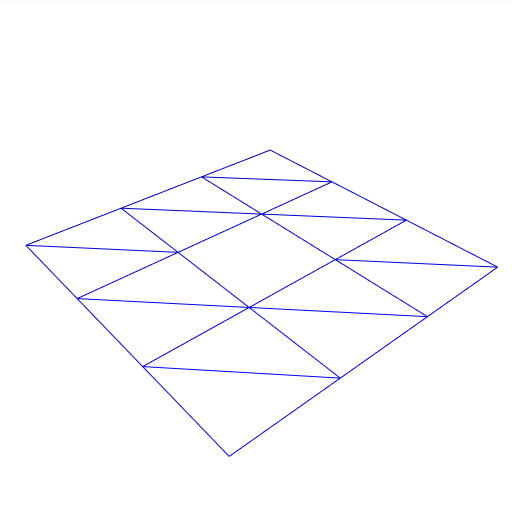
\includegraphics[trim={0 0 0 2cm},clip,width=0.95\textwidth]{images/model-ring-0.png}
          \caption{Ring}
        \end{subfigure}
        \begin{subfigure}[b]{0.24\textwidth}
          \center
          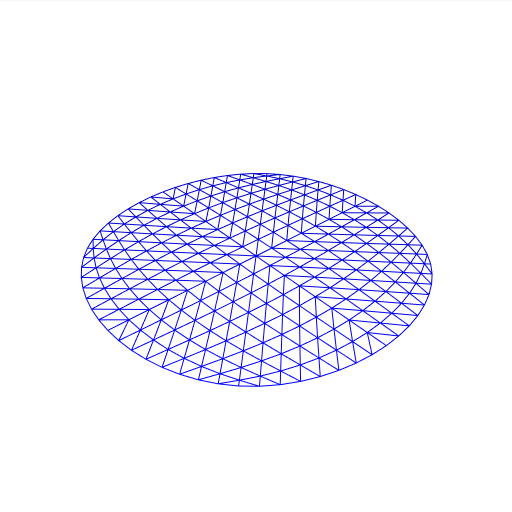
\includegraphics[trim={0 0 0 2cm},clip,width=0.95\textwidth]{images/model-circle-0.png}
          \caption{Curved}
        \end{subfigure}
        \begin{subfigure}[b]{0.24\textwidth}
          \center
          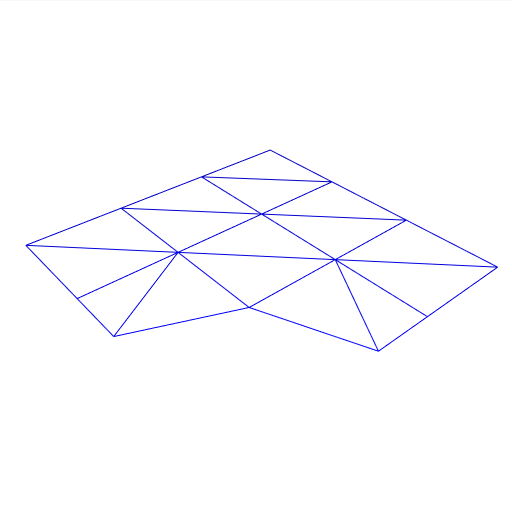
\includegraphics[trim={0 0 0 2cm},clip,width=0.95\textwidth]{images/model-test-0.png}
          \caption{Test}
        \end{subfigure}
      \end{figure}

      \begin{figure}[h]
        \begin{subfigure}[b]{0.24\textwidth}
          \center
          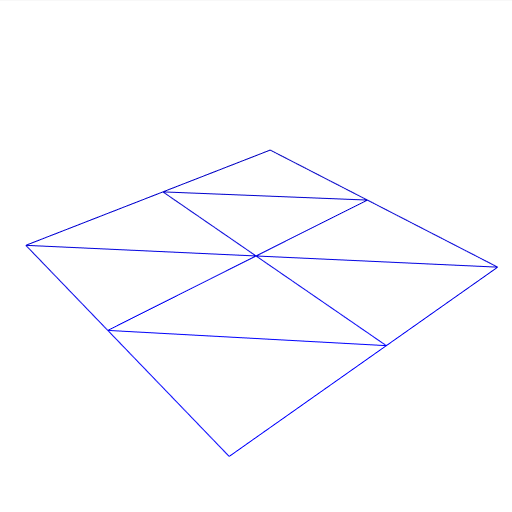
\includegraphics[trim={0 0 0 2cm},clip,width=0.95\textwidth]{images/model-quad-1.png}
          \caption{Quad}
        \end{subfigure}
        \begin{subfigure}[b]{0.24\textwidth}
          \center
          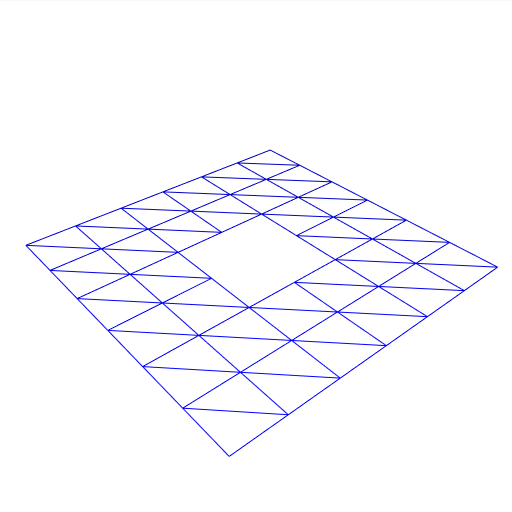
\includegraphics[trim={0 0 0 2cm},clip,width=0.95\textwidth]{images/model-ring-1.png}
          \caption{Ring}
        \end{subfigure}
        \begin{subfigure}[b]{0.24\textwidth}
          \center
          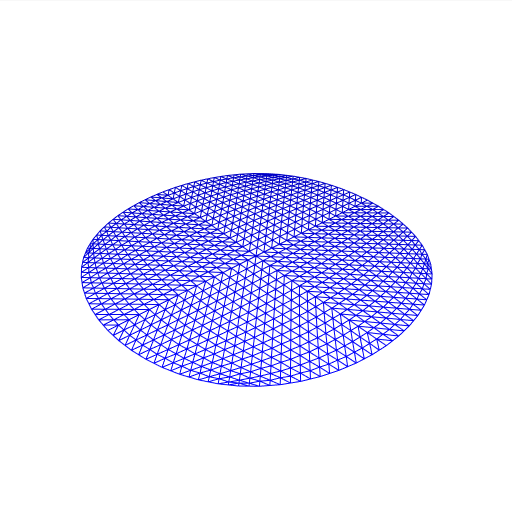
\includegraphics[trim={0 0 0 2cm},clip,width=0.95\textwidth]{images/model-circle-1.png}
          \caption{Curved}
        \end{subfigure}
        \begin{subfigure}[b]{0.24\textwidth}
          \center
          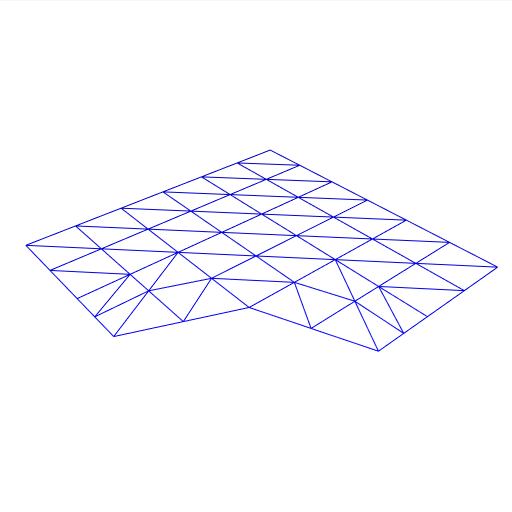
\includegraphics[trim={0 0 0 2cm},clip,width=0.95\textwidth]{images/model-test-1.png}
          \caption{Test}
        \end{subfigure}
      \end{figure}
    % subsection repräsentation_des_berechnungsgebietes (end)

    \subsection{Aufbau des Systems} % (fold)
    \label{sub:aufbau_des_systems}
      Ein System zur Lösung der Wellengleichung soll zunächst auf der CPU implementiert werden.
      Hierfür wird die Klasse \code{Cpu\_wave\_system} eingeführt.
      Sie verwendet die Bibliothek Eigen für alle grundlegenden Matrix-Vektor-Operationen.
      \inputCodeBlock[title=Wave system]{code/cpu_wave_system.cc}
      Das Interface des Systems besteht grundlegend aus einer Funktion \code{initial\_state}, die es ermöglicht die Anfangsbedingungen zu setzen, und einer Funktion \code{advance}, die das gesamte System einen Zeitschritt voranbringt.
      Systemmatrizen der Finite-Elemente-Methode sowie die Welle und deren Ableitungen werden zwischengespeichert, um unnötige Berechnungsschritte zu verhindern.
      Des Weiteren sollen bei der Konstruktion des Systems Eckpunkte, die auf dem Rand des Gebietes liegen, von den inneren Eckpunkten separiert werden.
      Hierfür wird das Array der Eckpunkte innerhalb des Systems permutiert.
      Die Permutation wird für den Zugriff von außen gespeichert.

      Auf der GPU ist die Verwendung von Eigen nicht möglich.
      Aus diesem Grund ist eine explizite Implementierung des CSR-Formates auf dem DRAM der GPU nötig.
      Um den Zugriff auf die Daten in CUDA zu ermöglichen, werden Zeiger definiert.
      Das Interface der Klasse \code{Gpu\_wave\_system} unterscheidet sich im Wesentlichen nicht von dem der Klasse \code{Cpu\_wave\_system}.
      Möchte man jedoch die Welle auslesen, so müssen deren Daten vom DRAM wieder in den RAM übertragen werden.
      Eben deshalb wird eine Funktion \code{copy\_wave} deklariert.

      \inputCodeBlock[title = GPU Wave system]{code/gpu_wave_system.cc}
    % subsection aufbau_des_systems (end)

    \subsection{Konstruktion der Systemmatrizen} % (fold)
    \label{sub:konstruktion_der_mass_und_stiffness_matrix}
      Die Konstruktion der Systemmatrizen muss in dieser für jedes Berechnungsgebiet nur ein einziges Mal ausgeführt werden.
      Aus diesem Grund soll hier auf die Implementierung einer parallelisierten Methode auf der GPU verzichtet werden.

      Für die Simulation der Wellengleichung werden vier Systemmatrizen benötigt.
      Diese teilen sich auf in die inneren Matrizen, die die Wechselwirkung freier Eckpunkte untereinander beschreiben, und Randmatrizen, die die Wechselwirkung des Dirichlet-Randes mit inneren Eckpunkten beschreiben.
      Zunächst werden die Eckpunkte auf einem Dirichlet-Rand markiert.
      Auf der Basis dieser Markierung lässt sich die Permutation konstruieren.
      In Anschluss daran, wird über die Dreiecke iteriert.
      Jedes Dreieck liefert die Matrix eines finiten Elementes.
      Diese Matrizen werden akkumuliert und zu den Systemmatrizen zusammengesetzt.
      \inputCodeBlock[title = System construction]{code/cpu_wave_system_constructor.cc}

      Für die GPU müssen die auf der CPU konstruierten Daten der dünnbesetzten Matrizen noch auf den DRAM übertragen werden.
      Dabei wird sich zu Nutze gemacht, dass die beiden inneren Matrizen das gleichen Muster besitzen.
      Ebenso gilt dies für die beiden Randmatrizen.
      Während der Konstruktion wird zudem die maximale Anzahl von Threads auf einem Block der verwendeten GPU ausgelesen.
      Mithilfe dieses Wertes wird eine optimale Anzahl von Threads auf den verschiedenen Blocks der GPU generiert.
      \inputCodeBlock[title = System construction]{code/gpu_wave_system_constructor.cc}

      Da die Daten auf dem DRAM über herkömmliche Zeiger verwaltet werden, muss der Destruktor der Klasse den allozierten Speicher auf dem DRAM wieder freigeben.
      \inputCodeBlock[title = System construction]{code/gpu_wave_system_destructor.cc}

      Die Funktionen, um die Anfangsdaten zu setzen und die Wellendaten auszulesen, müssen ebenfalls die Daten zwischen dem RAM und dem DRAM transportieren.
      \inputCodeBlock[title = System construction]{code/gpu_wave_system_accessors.cc}
    % subsection konstruktion_der_mass_und_stiffness_matrix (end)

    \subsection{Berechnung eines Zeitschrittes} % (fold)
    \label{sub:konstruktion_des_linearen_gleichungssystems}
      Die Berechnung eines weiteren Zeitschrittes erfordert die Konstruktion der rechten Seite des linearen Gleichungssystems.
      Mithilfe des in Eigen implementierten Conjugate Gradient Verfahren wird dann die Ableitung der Welle zum neuen Zeitpunkt berechnet.
      Anschließend kann mit dieser Ableitung die neue Welle generiert werden.
      \inputCodeBlock[title = CPU Wave System advance]{code/cpu_wave_system_advance.cc}

      Um den Lösungsalgorithmus auf der GPU zu programmieren soll zunächst das Conjugate Gradient Verfahren auf der CPU implementiert werden.
      Der folgende Quelltext zeigt dies.
      \inputCodeBlock[title = Conjugate Gradient]{code/cpu_conjugate_gradient.cc}
      Innerhalb der GPU wird nun genau wie auf der CPU zuerst die rechte Seite des linearen Gleichungssystems konstruiert und dann ein Conjugate Gradient Verfahren angewendet.
      Um die Implementierung einfacher zu gestalten, wurde Thrust verwendet.
      \inputCodeBlock[title = GPU Wave System advance]{code/gpu_wave_system_advance.cc}
      Innerhalb des Codes wird ein Kernel definiert, der die Matrix-Vektor-Multiplikation des CSR-Formates auf der GPU parallelisiert.
      Des Weiteren wurden zwei Funktoren \code{saxpy\_functor} und \code{saxpby\_functor} verwendet, die die typischen BLAS Routinen darstellen.
      \inputCodeBlock[title = GPU Kernel]{code/gpu_wave_system_kernel.cc}
    % subsection konstruktion_des_linearen_gleichungssystems (end)

    \subsection{Visualisierung} % (fold)
    \label{sub:visualisierung}

      Die Verwendung von OpenGL ermöglicht die dreidimensionale Darstellung von Objekten, die durch Dreiecke diskretisiert wurden.
      Um die Darstellung der Wellenfunktion und des Berechnungsgebietes noch anschaulicher zu gestalten, wurde jedem Eckpunkt des Gebietes als dritte Koordinate die Werte der Welle zugewiesen.
      Zudem wurde eine Farbverteilung berechnet.
      Die folgenden Abbildungen zeigen mehrere Beispiele.
      \begin{figure}[h]
        \center
        \begin{subfigure}[b]{0.24\textwidth}
          \center
          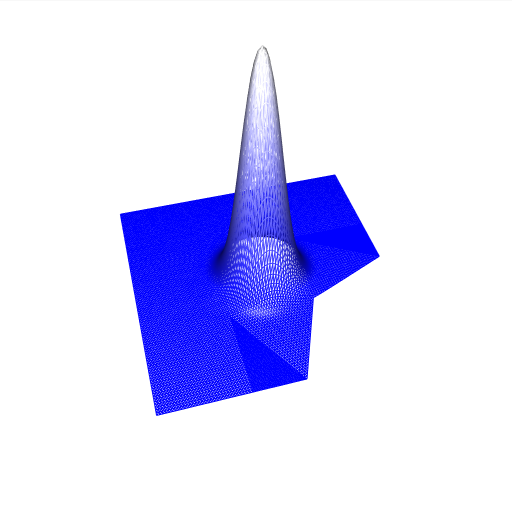
\includegraphics[trim={4cm 1.2cm 4.5cm 1.5cm},clip,width=0.95\textwidth]{images/test_wave_0.png}
          \caption{}
        \end{subfigure}
        \begin{subfigure}[b]{0.24\textwidth}
          \center
          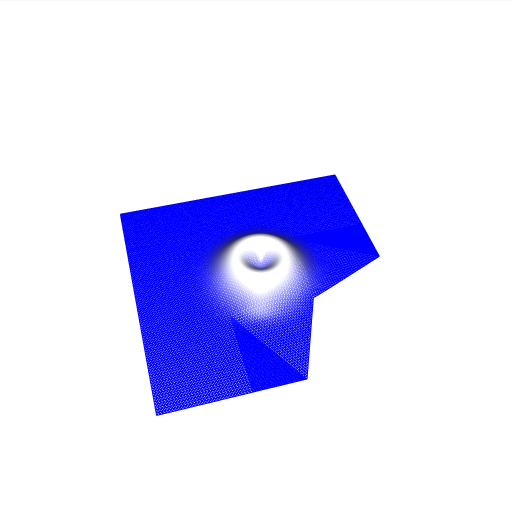
\includegraphics[trim={4cm 1.2cm 4.5cm 1.5cm},clip,width=0.95\textwidth]{images/test_wave_1.png}
          \caption{}
        \end{subfigure}
        \begin{subfigure}[b]{0.24\textwidth}
          \center
          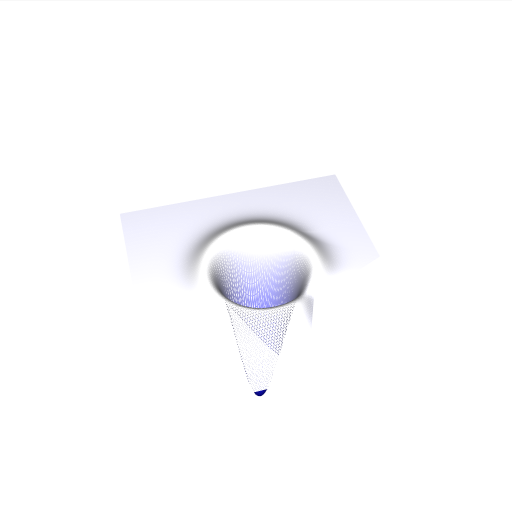
\includegraphics[trim={4cm 1.2cm 4.5cm 1.5cm},clip,width=0.95\textwidth]{images/test_wave_2.png}
          \caption{}
        \end{subfigure}
        \begin{subfigure}[b]{0.24\textwidth}
          \center
          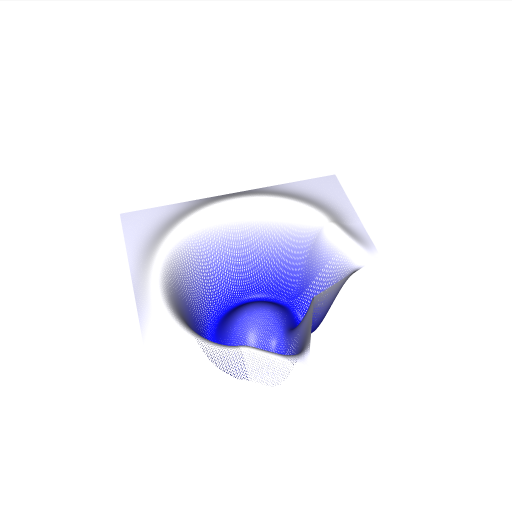
\includegraphics[trim={4cm 1.2cm 4.5cm 1.5cm},clip,width=0.95\textwidth]{images/test_wave_3.png}
          \caption{}
        \end{subfigure}

        \begin{subfigure}[b]{0.24\textwidth}
          \center
          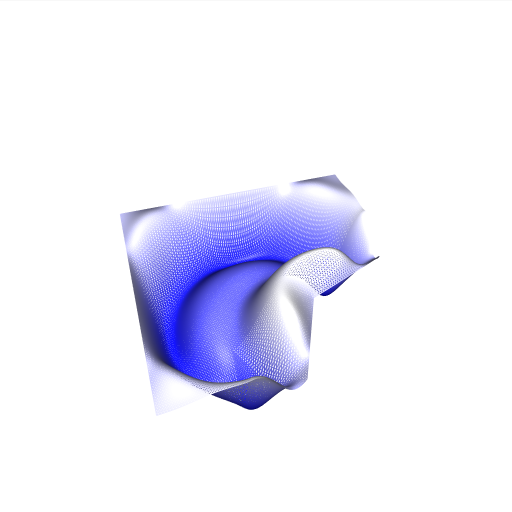
\includegraphics[trim={4cm 1.2cm 4.5cm 1.5cm},clip,width=0.95\textwidth]{images/test_wave_4.png}
          \caption{}
        \end{subfigure}
        \begin{subfigure}[b]{0.24\textwidth}
          \center
          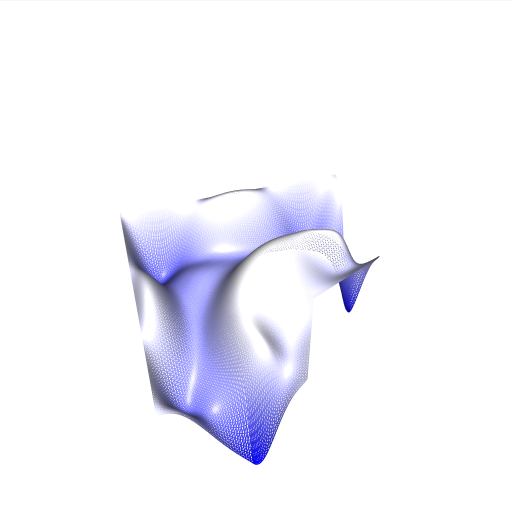
\includegraphics[trim={4cm 1.2cm 4.5cm 1.5cm},clip,width=0.95\textwidth]{images/test_wave_5.png}
          \caption{}
        \end{subfigure}
        \begin{subfigure}[b]{0.24\textwidth}
          \center
          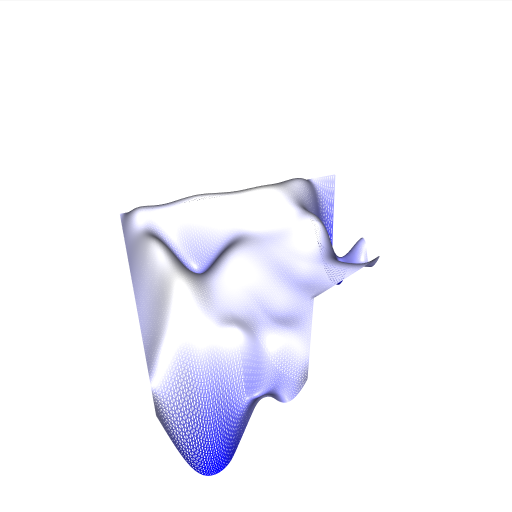
\includegraphics[trim={4cm 1.2cm 4.5cm 1.5cm},clip,width=0.95\textwidth]{images/test_wave_6.png}
          \caption{}
        \end{subfigure}
        \begin{subfigure}[b]{0.24\textwidth}
          \center
          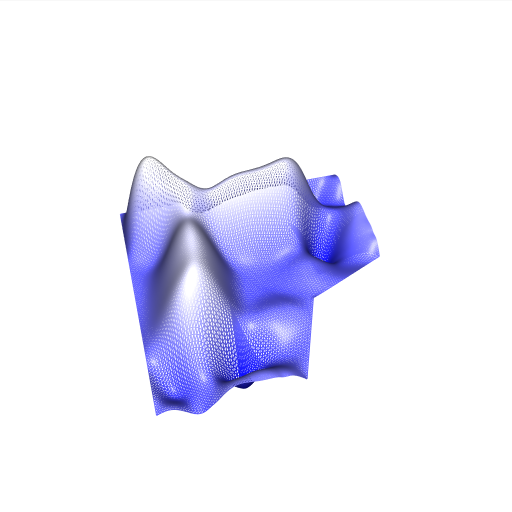
\includegraphics[trim={4cm 1.2cm 4.5cm 1.5cm},clip,width=0.95\textwidth]{images/test_wave_7.png}
          \caption{}
        \end{subfigure}
        \caption{}
        \label{fig:test-wave}
      \end{figure}

      \begin{figure}[h]
        \center
        \begin{subfigure}[b]{0.24\textwidth}
          \center
          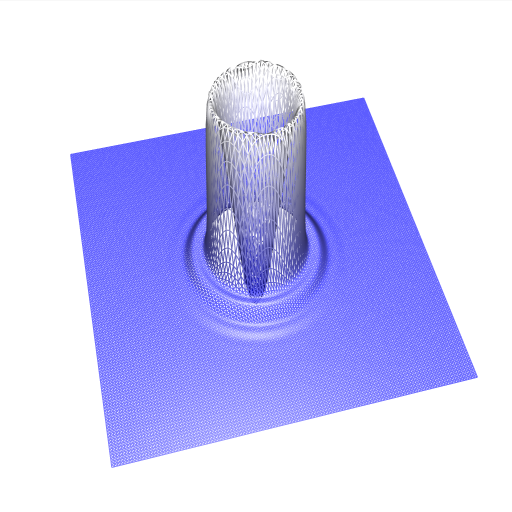
\includegraphics[trim={2cm 1.5cm 1.2cm 1.0cm},clip,width=0.95\textwidth]{images/quad_wave_0.png}
          \caption{}
        \end{subfigure}
        \begin{subfigure}[b]{0.24\textwidth}
          \center
          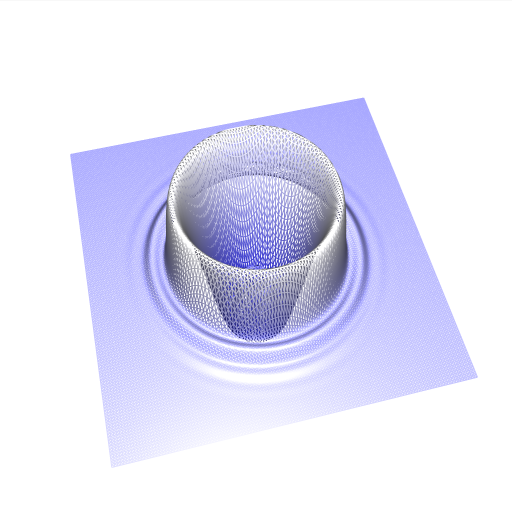
\includegraphics[trim={2cm 1.5cm 1.2cm 1.0cm},clip,width=0.95\textwidth]{images/quad_wave_1.png}
          \caption{}
        \end{subfigure}
        \begin{subfigure}[b]{0.24\textwidth}
          \center
          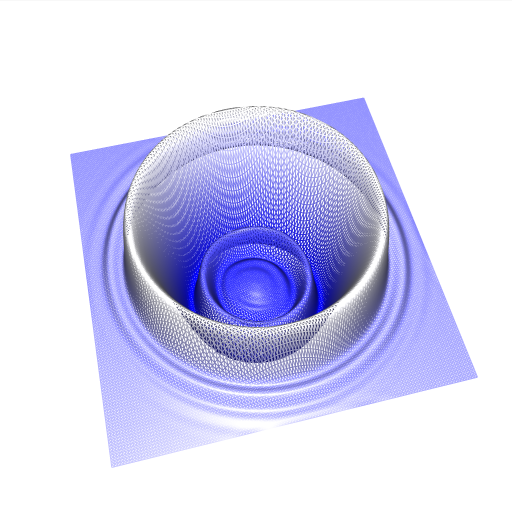
\includegraphics[trim={2cm 1.5cm 1.2cm 1.0cm},clip,width=0.95\textwidth]{images/quad_wave_2.png}
          \caption{}
        \end{subfigure}
        \begin{subfigure}[b]{0.24\textwidth}
          \center
          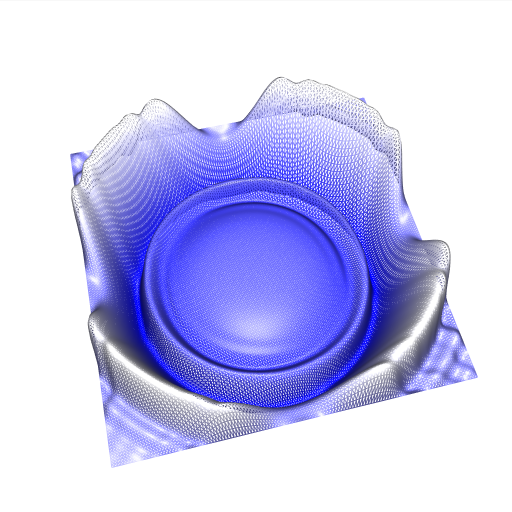
\includegraphics[trim={2cm 1.5cm 1.2cm 1.0cm},clip,width=0.95\textwidth]{images/quad_wave_3.png}
          \caption{}
        \end{subfigure}

        \begin{subfigure}[b]{0.24\textwidth}
          \center
          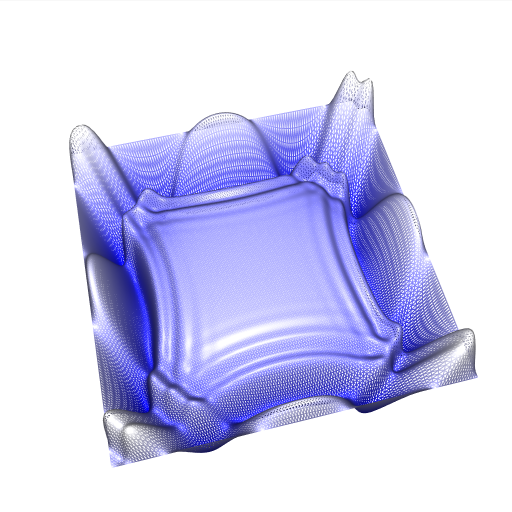
\includegraphics[trim={2cm 1.5cm 1.2cm 1.0cm},clip,width=0.95\textwidth]{images/quad_wave_4.png}
          \caption{}
        \end{subfigure}
        \begin{subfigure}[b]{0.24\textwidth}
          \center
          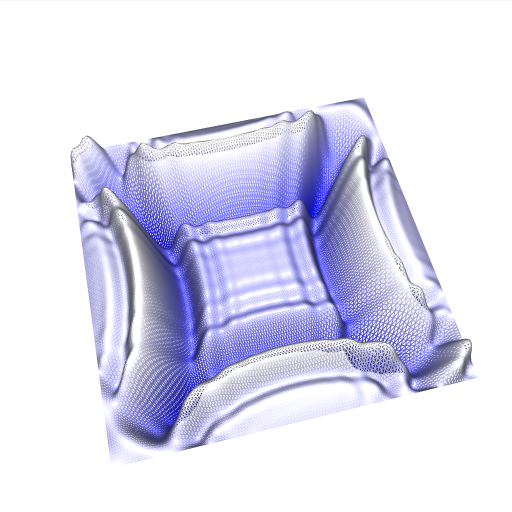
\includegraphics[trim={2cm 1.5cm 1.2cm 1.0cm},clip,width=0.95\textwidth]{images/quad_wave_5.png}
          \caption{}
        \end{subfigure}
        \begin{subfigure}[b]{0.24\textwidth}
          \center
          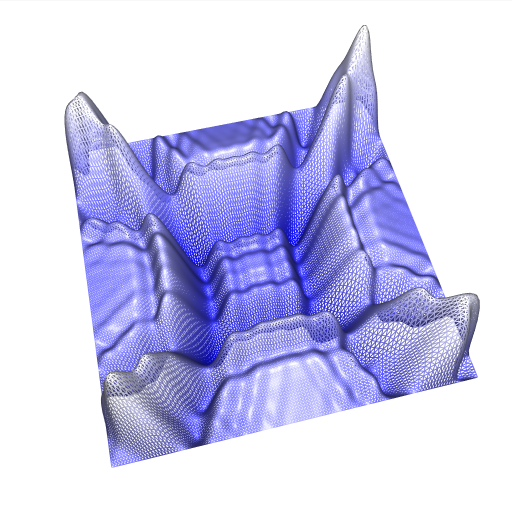
\includegraphics[trim={2cm 1.5cm 1.2cm 1.0cm},clip,width=0.95\textwidth]{images/quad_wave_6.png}
          \caption{}
        \end{subfigure}
        \begin{subfigure}[b]{0.24\textwidth}
          \center
          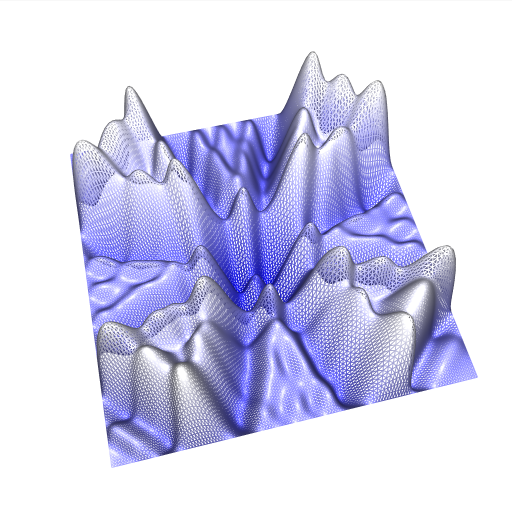
\includegraphics[trim={2cm 1.5cm 1.2cm 1.0cm},clip,width=0.95\textwidth]{images/quad_wave_7.png}
          \caption{}
        \end{subfigure}
        \caption{}
        \label{fig:test-wave}
      \end{figure}

      \begin{figure}[h]
        \center
        \begin{subfigure}[b]{0.24\textwidth}
          \center
          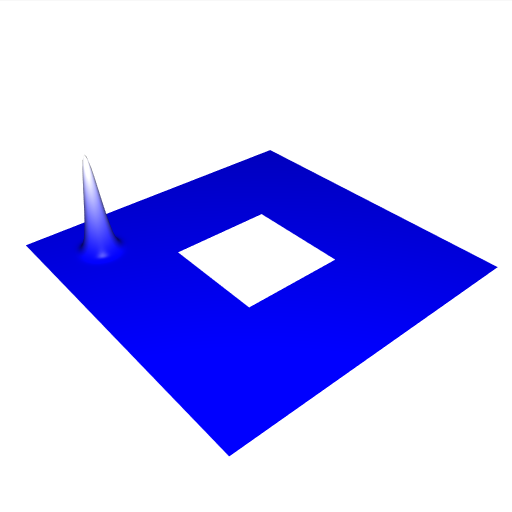
\includegraphics[trim={0.9cm 1.8cm 0.5cm 5cm},clip,width=0.95\textwidth]{images/ring_wave_0.png}
          \caption{}
        \end{subfigure}
        \begin{subfigure}[b]{0.24\textwidth}
          \center
          
\includegraphics[trim={0.9cm 1.8cm 0.5cm 5cm},clip,width=0.95\textwidth]{images/ring_wave_1.png}
          \caption{}
        \end{subfigure}
        \begin{subfigure}[b]{0.24\textwidth}
          \center
          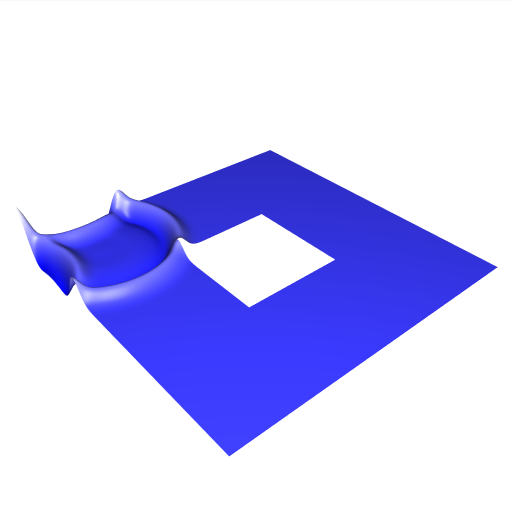
\includegraphics[trim={0.9cm 1.8cm 0.5cm 5cm},clip,width=0.95\textwidth]{images/ring_wave_2.png}
          \caption{}
        \end{subfigure}
        \begin{subfigure}[b]{0.24\textwidth}
          \center
          
\includegraphics[trim={0.9cm 1.8cm 0.5cm 5cm},clip,width=0.95\textwidth]{images/ring_wave_3.png}
          \caption{}
        \end{subfigure}

        \begin{subfigure}[b]{0.24\textwidth}
          \center
          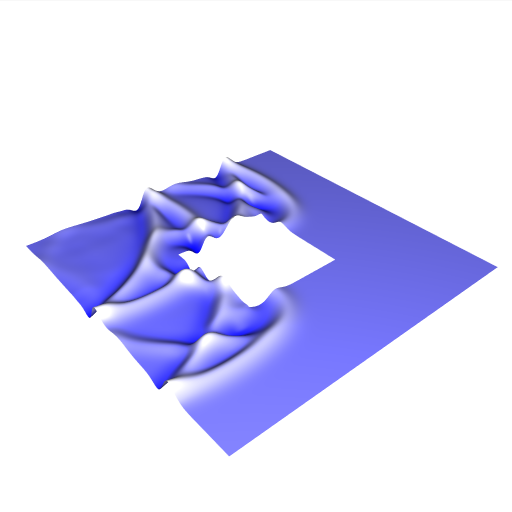
\includegraphics[trim={0.9cm 1.8cm 0.5cm 5cm},clip,width=0.95\textwidth]{images/ring_wave_4.png}
          \caption{}
        \end{subfigure}
        \begin{subfigure}[b]{0.24\textwidth}
          \center
          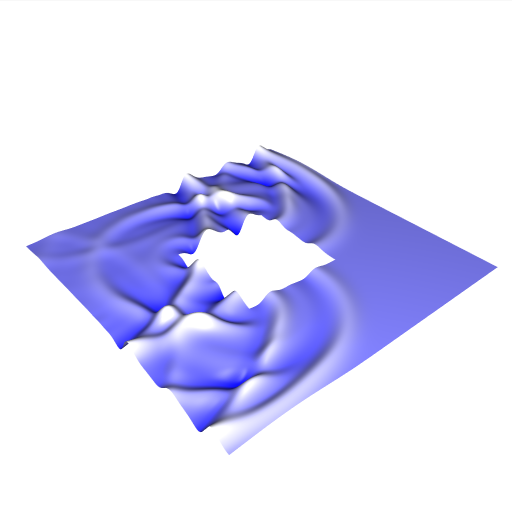
\includegraphics[trim={0.9cm 1.8cm 0.5cm 5cm},clip,width=0.95\textwidth]{images/ring_wave_5.png}
          \caption{}
        \end{subfigure}
        \begin{subfigure}[b]{0.24\textwidth}
          \center
          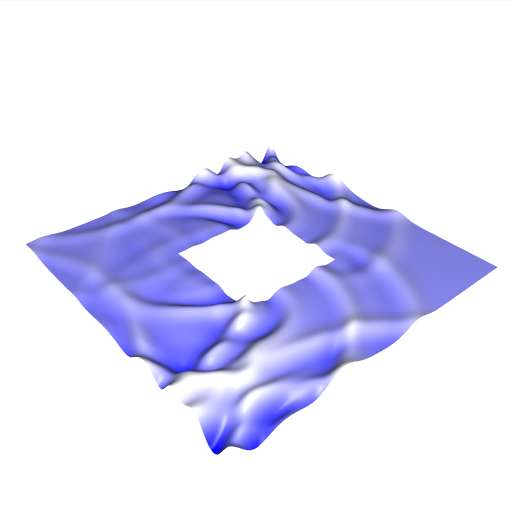
\includegraphics[trim={0.9cm 1.8cm 0.5cm 5cm},clip,width=0.95\textwidth]{images/ring_wave_6.png}
          \caption{}
        \end{subfigure}
        \begin{subfigure}[b]{0.24\textwidth}
          \center
          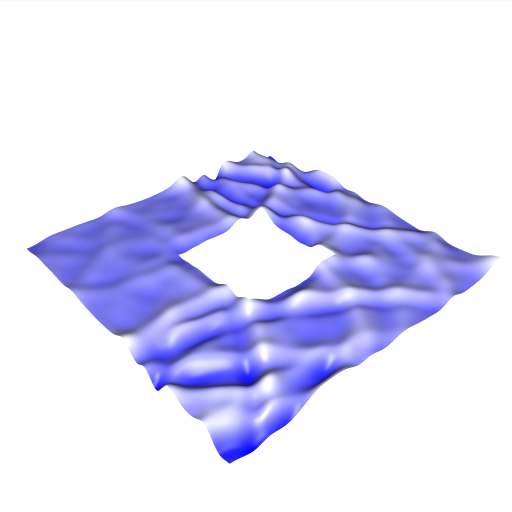
\includegraphics[trim={0.9cm 1.8cm 0.5cm 5cm},clip,width=0.95\textwidth]{images/ring_wave_7.png}
          \caption{}
        \end{subfigure}
        \caption{}
        \label{fig:ring-wave}
      \end{figure}

      \begin{figure}[h]
        \center
        \begin{subfigure}[b]{0.24\textwidth}
          \center
          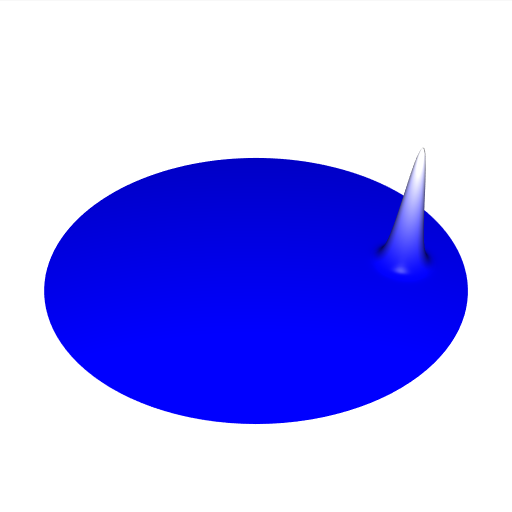
\includegraphics[trim={1.5cm 3.05cm 1.5cm 5.2cm},clip,width=0.95\textwidth]{images/circle_wave_0.png}
          \caption{}
        \end{subfigure}
        \begin{subfigure}[b]{0.24\textwidth}
          \center
          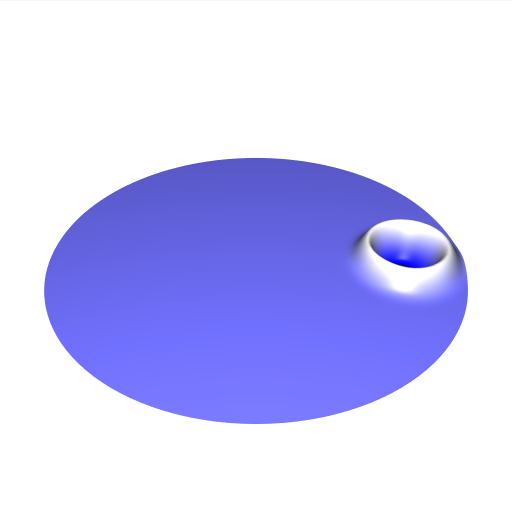
\includegraphics[trim={1.5cm 3.05cm 1.5cm 5.2cm},clip,width=0.95\textwidth]{images/circle_wave_1.png}
          \caption{}
        \end{subfigure}
        \begin{subfigure}[b]{0.24\textwidth}
          \center
          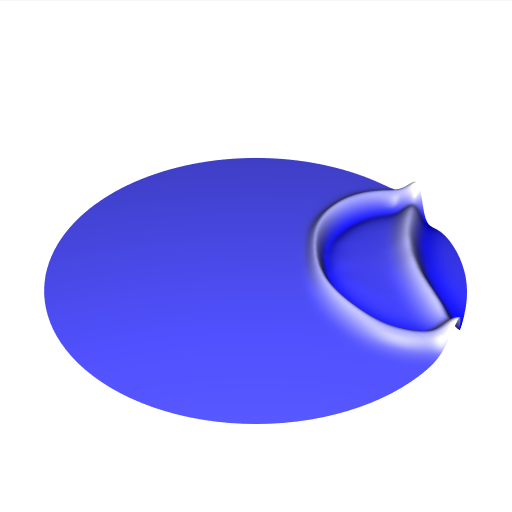
\includegraphics[trim={1.5cm 3.05cm 1.5cm 5.2cm},clip,width=0.95\textwidth]{images/circle_wave_2.png}
          \caption{}
        \end{subfigure}
        \begin{subfigure}[b]{0.24\textwidth}
          \center
          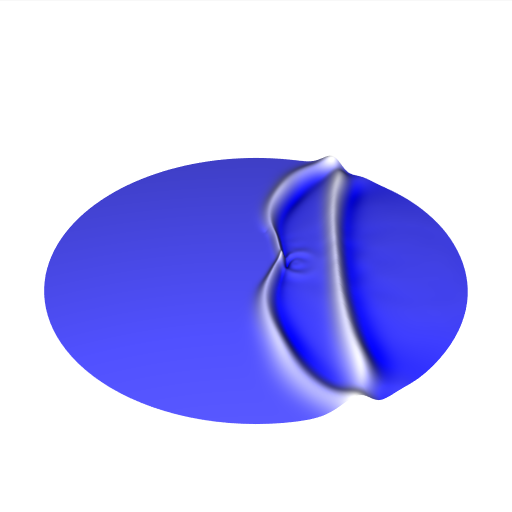
\includegraphics[trim={1.5cm 3.05cm 1.5cm 5.2cm},clip,width=0.95\textwidth]{images/circle_wave_3.png}
          \caption{}
        \end{subfigure}

        \begin{subfigure}[b]{0.24\textwidth}
          \center
          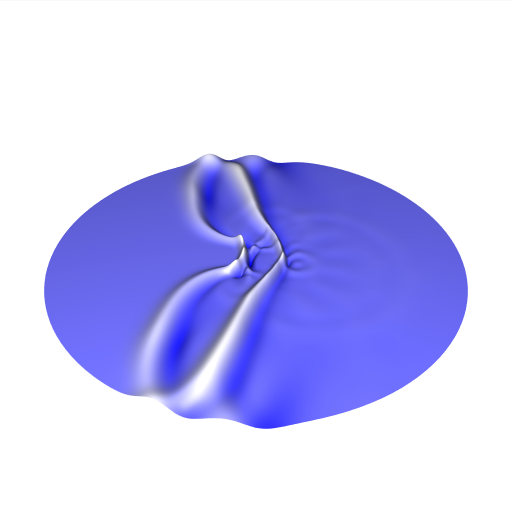
\includegraphics[trim={1.5cm 3.05cm 1.5cm 5.2cm},clip,width=0.95\textwidth]{images/circle_wave_4.png}
          \caption{}
        \end{subfigure}
        \begin{subfigure}[b]{0.24\textwidth}
          \center
          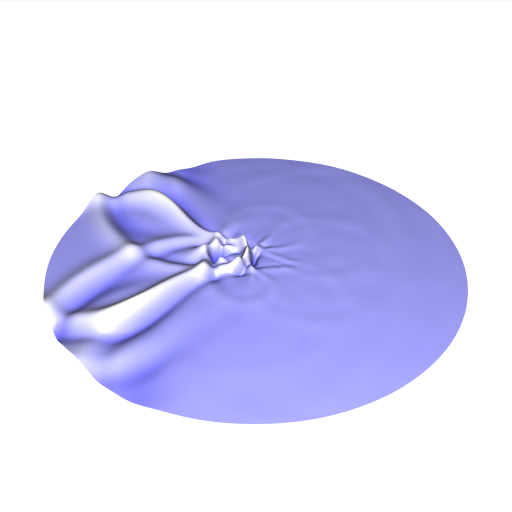
\includegraphics[trim={1.5cm 3.05cm 1.5cm 5.2cm},clip,width=0.95\textwidth]{images/circle_wave_5.png}
          \caption{}
        \end{subfigure}
        \begin{subfigure}[b]{0.24\textwidth}
          \center
          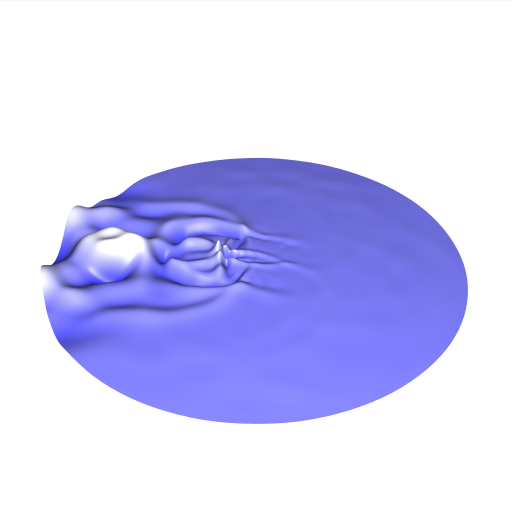
\includegraphics[trim={1.5cm 3.05cm 1.5cm 5.2cm},clip,width=0.95\textwidth]{images/circle_wave_6.png}
          \caption{}
        \end{subfigure}
        \begin{subfigure}[b]{0.24\textwidth}
          \center
          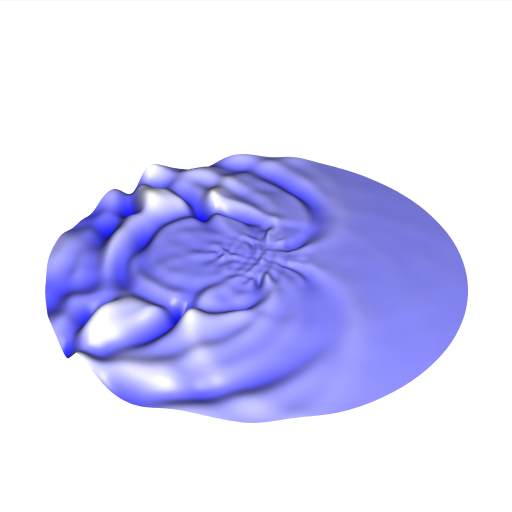
\includegraphics[trim={1.5cm 3.05cm 1.5cm 5.2cm},clip,width=0.95\textwidth]{images/circle_wave_7.png}
          \caption{}
        \end{subfigure}
        \caption{}
        \label{fig:circle-wave}
      \end{figure}

    % subsection visualisierung (end)
  % section implementierung (end)
\end{document}